\section{Adaptations to make sequential smoltcp amenable to 'distribution'}
\note{I might mention:
While this work was being conducted, smoltcp was being further developed. In particular, the device became an independent component. This logically moves the structure of the library in the direction we are aiming for. 
Therefore, we decided to use this new state of smoltcp as a further basis for the work and to adapt the previous changes accordingly. 
}

In this section we discuss, how our example application is composed using the original smoltcp API and how we need to transform the application itself, as well as smoltcp to make it amenable to compilation. 


\subsection{The initial situation}
In fact, there are two main aspects that need to be considered. The first is, that we need to present the compiler our target components and their basic interaction as stateful objects in the compile scope. It must be recognizable for the compiler, what the stateful components of the program are and how they interact. In particular, we must not as smoltcp currently does, give the device as a parameter to the TCP/IP component and let the later use the device 'under the hood', i.e. inside the library and outside the compile scope. The second aspect is, that all communication between components must be done explicitly via serializable messages, not via access to shared memory as before.

Figure~\ref{fig:oldTopLevel} shows a simple example of a server application using smoltcp. Obviously, this code does not meet our compilation requirements. Concrete problems are 
\begin{enumerate}
    \item Sockets are logically a part of the TCP/IP stack and should not appear in the compile scope
    \item In the call \rust{iface.poll} the state of an independent component, the device, is passed to the another component, the interface
    \item There are several direct accesses to the internal states of other components, e.g. in \rust{socket.listen(6969)} the application directly accesses a state of the TCP/IP stack
    \item States are not used linearly i.e. \todo[inline]{describe} 
\end{enumerate}


\begin{figure}[H]
    \centering
    
\begin{minted}[fontsize=\small]{rust}
fn main() {

    let mut store = Store::default();

    let mut device = TunTapInterface::new("tap0", Medium::Ethernet).unwrap();
    // ... more interface initialization code
    let mut iface = builder.finalize(&mut device);

    let mut sockets = SocketSet::new(vec![]);
    // .. more socket initialization code
    let tcp_socket = tcp::Socket::new(tcp_rx_buffer, tcp_tx_buffer);
    let tcp_handle = sockets.add(tcp_socket);

    loop {
        let timestamp = Instant::now();
        match iface.poll(timestamp, &mut device, & mut sockets) {
            Ok(_) => {}
            Err(e) => {
                debug!("poll error: {}", e);
            }
        }

        let socket = sockets.get_mut::<tcp::Socket>(tcp_handle);
        if !socket.is_open() {
            socket.listen(6969).unwrap();
        }

        if socket.may_recv() {
            let input = socket.recv(process_octets).unwrap();
            if socket.can_send() && !input.is_empty() {
                debug!(
                    "tcp:6969 send data: {:?}",
                    str::from_utf8(input.as_ref()).unwrap_or("(invalid utf8)")
                );
                let outbytes = store.handle_message(&input);
                socket.send_slice(&outbytes[..]).unwrap();
            }
        } else if socket.may_send() {
            debug!("tcp:6969 close");
            socket.close();
        }

        phy_wait(fd, iface.poll_delay(timestamp, &sockets)).expect("wait error");
    }
}
\end{minted}
    \caption{Simplified example of a server application using smoltcp}
    \label{fig:oldTopLevel}
\end{figure}


\subsection{The Goal}
So to better understand the required code changes we start at the top-level. How does the code we have seen in the previous section need to look like to produce the desired output program. Figure~\ref{fig:newTopLevel} illustrates the code we want to achieve. The first, and most trivial change is encapsulating initialization into \rust{init_<component>()} functions. This also entails encapsulating the sockets and the interface from the original code into one component.
\todo[inline]{refactor exapmle and add description when I know how I handle the socket handles}

Second we notice that each of our components is used only once in our target program. The function \rust{poll} that contains the interaction of  TCP/IP stack and the device to receive and send messages must become a pure function, i.e. taking both the TCP/IP stack and the device as arguments. We must lift it into compile scope and refactor the  usage of both components in the function to also follow our programming model. To enable this linear usage of states, we obviously need to transform the way those stateful components work in smoltcp. In Section~\ref{subsec:StateThreading} we further illustrate the problem and explain how to approach it.

Thirdly we see, that the communication between the components does not happen through mutual access to states anymore. For example, instead of accessing a socket directly via \rust{let socket = sockets.get_mut::<tcp::Socket>(tcp_handle);} we need to implement a data format and a command interface in both the \rust{app} component and the \rust{tcp_ip_stack} to enable such interactions via message passing. We discuss this issue in Section~\ref{subsec:MessagePassing} and present our implementation as a possible solution.

\begin{figure}[H]
    \centering
    
\begin{minted}[fontsize=\small]{rust}
fn main() {
    let mut app = init_app();
    let device = init_device();
    let (mut tcp_ip_stack, socket_handle) = init_tcp_ip_stack(device);
    // Contains: Actual payload messages for the sockets i.e. like {handle:[msgs]} and socket state information
    let socket_proxy_state = init_socket_proxy();
    while true {
        let states_n_data = poll(tcp_ip_stack, device, socket_proxy_state);
        let processed_data:CommandsAndMessages = app.do_your_thing(states_n_data);
        socket_proxy_state.update_all(processed_data) 
    }
}
\end{minted}
    \caption{To enable Ohua to extract a data flow graph with local states we need to lift the envisioned stateful components 'app', 'tcp\_ip\_stack' and 'device' and their interaction into compile scope as shown here.}
    \label{fig:newTopLevel}
\end{figure}

Finally we have to use a recursion instead of a \rust{while} loop. This is a current restriction of Ohua which we discuss in more detail in Section~\ref{subsubsec:WhileLoops}. 
\note{Note to me: Ohua also supports 'endless' for loops. However we have no way of gracefully ending them as we a) can not access the loop generator while running and b) we do not support early returns i.e. \rust{break} or \rust{return}}
\todo[inline]{figure out recursion}



\subsection{Transformations needed for state threading}
\label{subsec:StateThreading}
\todo[inline]{Adapt to better fit in the general flow}

In a sequential, single threaded program we can invoke a function on one 'component A', do something on it's state, call a function on another 'component B' and finish the outer call by maybe changing 'A's state again. This is what happens, when a packet is send or received using smoltcp in its current form. However in a concurrent, distributed data flow graph, we can not realize this bi-directional dependency among stateful components. Why is that? The main problem here is realizing concurrency and state locality at once. We could connect distributed components A and B using blocking connections, i.e. A calls B and blocks until it receives the result. What we achieve this way is a distributed, sequential program. Another way would be to have A send its state along with the call to B and B would return this state along with its answer. So A can process the next input and upon receiving an answer it can resume the appropriate state. However, this contradicts the requirement of state locality. In particular when states are large objects e.g. a database state, a training state of a deep neural network or alike, we want them to stay encapsulated in on component.\\

So to distribute the components of smoltcp, we need to disentangle state dependencies from each other. In the following subsection, we explain how this can be done using the TCP/ipv4 implementation of smoltcp. We will look in particular on how our envisioned components 'application', 'tcp/ip stack' and 'NIC' are connected during packet sending, receiving and finally in the \rust(poll()) call, that connects both. For each of those processes we will discuss how to transform the implementation of smoltcp, to extract a data flow graph using Ohua. 
\todo[inline]{Refer to linear State use here when the according background section is ready}


\subsubsection{Sending a Packet}
Figure~\ref{subfig:egressOrig} depicts a simplified control flow during the sending a package, in particular the \code{TCP/IP} component actually represents a nested structure and function calls. The point is however, that when our envisioned component \code{APP} call our envisioned component \code{TCP/IP} which in turn calls \code{NIC}, the callers have to keep their state and block execution until the callees return. This will not be the case, when we deploy those components as part of a data flow graph. In this case, each of the components will process any input based on its state output a result and wait for the next input. So we basically need the components to 'stream process' data. The second Figure~\ref{subfig:egressTransf} illustrates, how this can be done in our example. The forward pass of the call is basically the same as before, but we introduce conditionals to gate the data flow down the stack. The backward pass returning the result of sending is processed not by returning to the pre-call stack position, but also by explicitly passing a message through the components again. 
\todo[inline]{Describe where the if's belong to, mention order is preserved.}


\begin{figure}[H]
    \centering
    
\begin{minted}[fontsize=\small]{rust}
// interface.rs
fn socket_egress(&mut self) -> Result<bool> {
    /* get references to  device, inner_interface and sockets
       hold by the interface struct
       iterate sockets -> socket
       ask inner_interface if socket can egress
    */
    ...
        
        let mut device_result = Ok(());
        let socket_result = socket.dispatch(
                inner, 
                |inner, resp| {
                    let response = IpPacket::Raw(response);
                    neighbor_addr = Some(response.ip_repr().dst_addr());
                    let tx_token = device.transmit().ok_or(Error::Exhausted)?;
                    device_result = inner.dispatch_ip(tx_token, response);
                    device_result
                    }
            );

        match (device_result, socket_result) {
            // Error handling ...
        }
    // if any packet has been send:
    Ok(emitted_any)
}
\end{minted}
    \caption{Simplified code of the \rust{Interface.socket_egress} method}
    \label{fig:egressCode}
\end{figure}

\begin{figure}[H]
    \centering
\begin{minted}[fontsize=\small]{rust}
// tcpsocket.rs
pub(crate) fn dispatch<F>(&mut self, inner: &mut InterfaceInner, emit: F) -> Result<()>{
    /* check socket state using the inner interface
       maybe reset socket state and/or return an ErrExhausted
    */
    ...
    // build IP representation
    let mut ip_repr = 
    // build TCP representation
    let mut tcp_repr = 
    // set fields of the tcp packet, based on socket state and
    // inner state, adapt ip packet (payload len)
    ...
    // This calls the closure from outer scope
    emit(inner, (ip_repr, tcp_repr))?;
    
    // If this point is reached, emitting succeeded and
    // socket state is updated based on the tcp_repr send e.g.
    ...
    self.remote_last_ack = repr.ack_number;
    
    
}
\end{minted}
    \caption{Simplified code of the \rust{socket.dispatch} method}
    \label{fig:dispatchCode}
\end{figure}

\begin{figure}[H]
\centering
\tabskip=0pt
\valign{#\cr
    \hbox{%
    \begin{subfigure}{.3\textwidth}
    \centering
     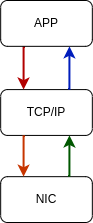
\includegraphics[height=5cm]{figures/egress_original_simple.png}
     \caption{Original flow of a packet sending call}
     \label{subfig:egressOrig}
    \end{subfigure}%
  }
  \cr
  \noalign{\hfill}
    \hbox{%
    \begin{subfigure}{.65\textwidth}
    \centering
    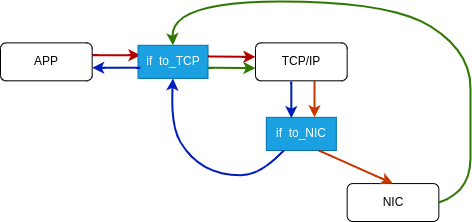
\includegraphics[height=5cm]{figures/egress_new_simple.png}
     \caption{Refactored control flow of the egress function call}
     \label{subfig:egressTransf}
    \end{subfigure}%
  }
  \vfill
  \cr
}
\caption{Transformation of the packet sending control flow to achieve state locality}
\label{fig:TransformEgress}
\end{figure}


\subsubsection{Receiving a Packet}

Just like sending, receiving is triggered in the \rust{Interface::poll()} method. In the \rust{Interface.socket_ingress()} method, a while loop receives packages form the device as long as there is a next package available. The main aspects of \rust{Interface.socket_ingress()} are depicted in Figure~\ref{fig:socketIngressCode}, lengthy parts are abbreviated by \rust{/**/}comments describing their effects.
Each packet is then 'unwrapped' from its protocol layers Ethernet and IP by the Inner Interface and redirected to the appropriate socket.  This may change the state of the Interface e.g. adding new sender IP addresses. The socket processes the package, again this is a state changing operation and returns a result that may contain an answer packet. If so, this packet is wrapped into an IP packet and Ethernet Frame by the Interface and forwarded to the device for sending. Otherwise, successful processing of a package just sets the \rust{processed_any} flag to let the calling application know that socket states have changed due to received packets.  

\begin{figure}[H]
    \centering
\begin{minted}[fontsize=\small]{rust}
fn socket_ingress(&mut self) -> bool {
    /*get references to sockets, inner and device*/
    
    // try to receive a data buffer object (rx_token) 
    // and a file handle to the device (tx_token)
    while let Some((rx_token, tx_token)) = device.receive() {
        // rx_token.consume applies the closure to the received data frame
        if let Err(err) = rx_token.consume(inner.now, |frame| match
            inner.caps.medium {
                /* matching for different medium, but we only care for 
                   Ethernet for now
                */
                // process_ethernet: remove protocol layers, direct package to socket
                Medium::Ethernet => match inner.process_ethernet(sockets, &frame) {
                    Ok(response) => {
                        processed_any = true;
                        // maybe socket answers directly with a packet
                        // e.g. with an ACK 
                        if let Some(packet) = response {
                            // package the packet in a frame and send
                            if let Err(err) = inner.dispatch(tx_token, packet) {...}
                        }
                        Ok(())
                    }
                },
                ...
            }) {net_debug!("Failed to consume RX token: {}", err);}
        processed_any
    }
\end{minted}
    \caption{Simplified code of the \rust{Interface.socket_ingress()} method}
    \label{fig:socketIngressCode}
\end{figure}

\todo[inline]{Describe While Loop: I can extend this to the appropriate 'while construct' by using the first case distinction as the while condition. What I still need to account for is the "processes any" flag. It can be transported along from TCP/IP to NIC to APP inside the NICCommand: MaybeSend() and the NICResult: Send().}
\todo[inline]{Where are Errors handled? 
\means All errors are caught and handled inside the loop i.e. it is sufficient to $OR$ the NICResult : Send() in every round. }
\todo[inline]{Actually there is another if-split between TCP/IP deciding whether to loop again or to go to the NIC for sending.}

\begin{figure}[H]
\centering
\tabskip=0pt
\valign{#\cr
    \hbox{%
    \begin{subfigure}{.3\textwidth}
    \centering
     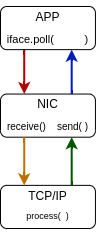
\includegraphics[height=5cm]{figures/ingress_simple_original.png}
     \caption{Original flow of a packet receiving call}
     \label{subfig:ingressOrig}
    \end{subfigure}%
  }
  \cr
  \noalign{\hfill}
    \hbox{%
    \begin{subfigure}{.65\textwidth}
    \centering
    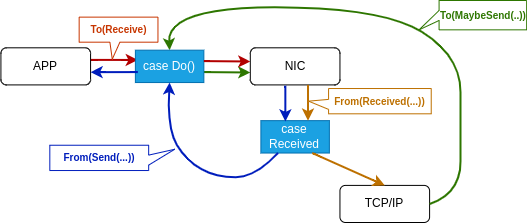
\includegraphics[height=5cm]{figures/ingress_simple_transformed.png}
     \caption{Refactored control flow of the ingress function call. Figure~\ref{fig:messageEnums} shows the new data types used to annotate the arrows.}
     \label{subfig:ingressTransf}
    \end{subfigure}%
  }
  \vfill
  \cr
}
\caption{Transformation of the packet receiving control flow to achieve state locality}
\label{fig:TransformIngress}
\end{figure}


\begin{figure}[H]
    \centering
\begin{minted}[fontsize=\small]{rust}
enum NICResult {
	Send(Result<T , Err>),
	Received(Result<Data, Err>)
} 

enum ToOrFrom {
	To(NICCommand),
	From(NICResult)
} 

enum NICCommand {
	Receive,
	MaybeSend(Option<Package>)
} 
\end{minted}
    \caption{Possible implementations for message formats among the components}
    \label{fig:messageEnums}
\end{figure}


\subsection{Transformations needed for Message Passing}
\label{subsec:MessagePassing}
As explained before the nodes of the DFG in the compiled program cannot access shared memory. So we need to extract the communication relations that rely on direct state acccess and transform them into message passing communication. For example, a server application (later application component), can directly create sockets (later network stack component), query their state and change it. \\


How to
\begin{enumerate}
    \item Zugriffe identifizieren ... im Zweifel erstmal für unsere Beispielanwendung
    \item Identifier für die Komponenten des Zustands (Sockets, inner interface, whatever) einführen, die serialisiert werden k\"onnen und eine gemeinsame Sprache der kommunizierenden Komponenten erm\"oglichen 
    \item Aus allen identifizierten Interactionen ein Nachrichtenformat entwickeln um diese abzubilden \means einfachste Variante ist serialisierung der funktionsaufrufe
    \item Das "Zustands-kapselungs-paradigma" erzwingt soweit ich das sehe eine zentrale "Schnittstelle" pro Komponente, die die eingehenden Nachrichten verarbeitet
    \item Wenn ferig \means kann man das Vorgehen generalisieren/automatisieren
\end{enumerate}


\note{Da die Sockets jetzt nicht mehr Teil des Interfaces sind gibt es mehrere grunds\"atzliche M\"oglichkeiten: 

Ich weiss noch nicht ob es eine automatische/generelle M\"oglichkeit der Ableitung gibt, aber das sieht aus wie Domain-Knowledge \means Programmers Responsibility
}
M\"oglichkeiten:
\begin{itemize}
    \item Man k\"onnte tats\"achlich die Sockets rumschicken, dh. das SocketSet als daten Betrachten 
    \item Man k\"onnte eine vollst\"andige Representation der Sockets auf beiden Seiten haben
    \item app hat eine vereinfachte Version der Sockets mit State und Commands \means wenn man es genau auf eine Anwendung zuschneiden will, k\"onnte man alle \rust{socket.is_something()} Zugriffe identifizieren, die muss der abgeflachte zustand beanworten k\"onnen, und alle \rust{socket.do_something()} Zugriffe identifizieren, die m\"ssen als commands vom Interface verstanden werden. \means Um das sauber zu unterscheidnen muss man den Code der Funktionen untersuchen. Ich weiss nicht ob die Unterscheidung m\"oglich und sinnvoll ist und selbst wenn, ob /wie man z.B. bedingte Zugriffe \rust{if !socket.is_open() {socket.listen(6969).unwrap();}} umsetzen würde. 
\end{itemize}


\textbf{Steps for App-Interface:}
1. The most complex interaction (if not the only one) we need to tackle is the one between the app and the tcp\_ip\_stack. In the new smoltcp implementation, the sockets are a separate entity although they are logically a part of the tcp\_ip\_stack obviously. The app needs to be able to set up and identify sockets to manage connections, map requests and answers and so on. The interface needs the sockets to process incoming and outgoing packets based on their internal state.   




\subsection{Can we generalize?}
Observations
\begin{itemize}
    \item Which components should the program have? \means Could not be deduced from Code \means Domain knowledge of the programmer
    \item How to implement message passing? \means I currently suspect this is also a matter of domain knowledge 
    \item How to transform to linear state usage \means Firstly wee need to know the components. Second we'd need to follow their states in the code. However this probably entails knowing a) which encapsulated object (e.g. socket) belongs to the component and which one doesn't. Assuming the composed states are defined by the programmer we can follow their fields though function calls. We would assume correct code AND no keyword args as in Python so we can follow object using their position in a function call even if they're named differently inside the function \means we need to track aliasing \means this works as long as we can follow all calls i.e. no function calls to outside compile scope takes our objects as arguments \means I have to evaluate against our restrictions if referencing can get our objects can get in our way.
\end{itemize}


\subsection{other stuff}
\todo[inline]{Rewrite with examples}
\begin{itemize}
    \item Panics \means Errors are forwarded, meaning we can react on them in distributed settings, \rust{panic!} can in the M3 scenario at most be detected by the node sending to the panic node because M3 will notify a sender when the receiver is closed. In this scenario, the usual message path through the graph is obviously broken so the only way to propagate this would be an extra channel each node has to the main thread.
    \item currently only tuples of exactly 2 elements are supported \means either I adapt Ohua, or I need to introduce further wrapping for any more complex pattern
    \item currently input to functions i.e. parameters can not directly be used as stateful objects \means I need to introduce wrapper function calls, I might remove them in the backend again.
\end{itemize}

\section{Adaptations to make Ohua fit for relevant applications}
\subsection{Providing full type annotations}
Although Rust is a strongly typed language, type annotations for local variables are often unnecessary, since they are automatically derived from the type inference of the rust compiler. In contrast, definitions of types, i.e. structs, enums and functions, are the basis of type inference and must be annotated manually/by the programmer. Since Ohua produces new code in the backend, it is not enough to transfer existing annotations of the input to the output. In particular, the communication channels of the produced tasks require type annotations, since these cannot be completely derived by the Rust type inference even in the shared memory scenario. Also in view of a later extension to fully distributed systems, distributed compilation of individual components or the use of languages with less powerful inference, it is important not to rely on the type inference specific to the compiled language. 

So where do we get the type information we need? One important observation is that Ohua does not create new types. The control functions Ohua inserts into the data flow graph are mainly there to pass on existing intermediate results of the original program. That is, the types of these functions that is, of their input and output channels can be derived from the input code. For this we need a) a type extraction from the input program and b) a type propagation which propagates the corresponding types through the representation of the data flow graph. Both were basically available at the beginning of the work. However, the existing implementation had problems or was not fully functional. This means that some types had to be annotated by hand in the output code. The following sections describe how type extraction and type propagation worked and which changes were necessary to achieve the desired functionality. \\

\subsubsection{Type Extraction}
So the first functionality we had to address was the \code{Type Extraction} in the frontend integration. Until now this was a two step process. In a first pass two kinds of data were extracted from the input module. One was the algorithms i.e. the Rust functions that were to be compiled. Those were translated to an internal representation of the supported Rust subset as described in Section~\ref{subsec:RustIntegration}. The second structure kept track of imports defined in the module. \\

The second pass was needed to annotate types to function names. As each function call \rust{let z = someFun(x, y);} might become an independent node, the compiler needs type annotations for \rust{x} and \rust{y} to later annotate the channels for sending those variables among independent tasks. To do so first the function names called in the parsed algorithms were extracted. Then all files defined in the imports where scanned for function definitions. From this information, a hashmap was built over all function names and the extracted function types. Finally, in a further traversal over the input code, this hashmap was used to lookup function types and annotate them in the input code. This procedure had some disadvantages, namely : 

\begin{itemize}
    \item The entire compile scope, including for example the standard library, had to be available for the compiler to find and process. This introduced path dependencies of the compiler and notably excludes the import of compiled libraries in other languages e.g. libc, which is critical in our case.
    \item We had to restrict the entire compile scope and imported libraries to syntax the compiler could understand. This has previously been addressed by re-implementing some required libraries in a simpler form. 
    \item We had to keep track of name spaces and aliasing for all functions
    \item We could not support 1. generic type parameters in function definitions and 2. overloaded function definitions.
\end{itemize}

The main point of concern was really the need to parse the whole scope and therefore to have all libraries used available and compatible to Ohua supported syntax. Therefore we chose to change the source of type information. Instead of collecting function signatures from the scope and typing functions globally for the complied module, we now type each call site according to the local context. Remember, we need to type the input parameters for each function call inside an algorithm. Those parameters can be: 

\begin{itemize}
    \item global constants, in which case Rust requires a type annotation
    \item input parameters of the algorithm, in which case we know their type from the algorithm signature
    \item local variables bound in the algorithm, in which case we now require the programmer to provide type annotation 
\end{itemize}

So for most syntax constructs, we can derive the type information needed from the local context. This requires the programmer to annotate types manually in local assignments, where it would not be required by Rust itself. Also Figure~\ref{fig:TypeExtractionExample} shows an example, where additional local bindings are required. In the example code, to be able to type the function call to \rust{h(e)} we need an additional binding statement as it is not possible to type annotate a loop pattern currently. 

\begin{figure}[H]
\centering
\tabskip=0pt
\valign{#\cr
    \hbox{%
    \begin{subfigure}{.35\textwidth}
    \centering
     \begin{minted}[fontsize=\footnotesize]{rust}
fn test(i:i32) ->  {
    let s = State::new_state();
    for e in range_from(i) {
        let r = h(e);
        s.some_method(r);
    }
    s
}
     \end{minted}
    \end{subfigure}%
  }
  \cr
  \noalign{\hfill}
    \hbox{%
    \begin{subfigure}{.62\textwidth}
    \centering
    \begin{minted}[escapeinside=||,fontsize=\footnotesize]{haskell}
fn test(i:i32) -> () {
    let s:State = State::new_state();
    for e in range_from(i) {
        let e1:i32 = e;
        let r:i32 = h(e1);
        s.some_method(r);
    }
    s
}
    \end{minted}
    \end{subfigure}%
  }
  \vfill
  \cr
}
\caption{To extract type information for function call from the local context we require the  programmer to annotate the according types to local variables. As shown in the right code example it is sometimes also necessary to have additional binding statements to annotate every relevant variable i.e. every input to a function call.}
\label{fig:TypeExtractionExample}
\end{figure}

However, the new \code{Type Extraction} works without the need to parse the imported files. As we only type the concrete function call sites, this also allows the use of generically typed.\\
\todo[inline]{Check with felix whether and how this was a problem anyways since Ohua is perfectly fine with generics and also Rustwise it should be ok to infer at compiletime as usual}

The main change, required to implement this solution was threading a monadic context through the complete process of transforming the input code to the frontend representation. In particular also through the first step of this process, where the Rust code is mapped to a subset of Rust supported by Ohua. These context keeps track of variable bindings and according types in the current scope. In the outermost scope i.e. the global level of the input code, this context is pre-filled with constant definitions, including all global constant definitions parsed before the actual algorithms. 

The conversion of algorithms is also monadic process and the initial context contains the names and types extracted from the global scope. For each algorithm the parameter names and their types are parsed from the signature and added to the context. Upon parsing the body of the algorithm each right hand side of a let binding\footnote{We currently only support variable or tuple patterns} is checked for type annotation and registered in the local context if annotated properly. Unannotated bindings will yield an error at this point. AS shown in the example in Figure~\ref{fig:TypeExtractionExample} this might require some additional local assignments, when local variables result from pattern binding.\\

Now, whenever a function call is converted, the function type is derived from its arguments. In the case of a stateful call, this also includes the called object. If the arguments are variables, the types are obtained from the context. If the variables are not in the context, again an error is thrown. For supported literal arguments (currently integers, booleans and strings) the types are derived automatically. Obviously, this limits the accepted input syntax in that only literals and variables are valid as direct function arguments. Still the advantage of being able to use the entire Rust syntax again in the imported libraries outweighs this in our opinion. As function types now depend on the types of local variables we added test cases to the regression test suite to ensure proper typing, when local scope variables shadow names from outer scopes. Notably name shadowing inside the same scope is currently not supported by Ohuas renaming algorithm and could therefore not be tested.\\

\todo[inline]{Check where the below comments belong}
\note{Finally there are some open question we need to address regarding accepted types. Currently the type extraction mechanism just wraps any relevant type annotation from the input code in a to an internal argument type representation. This means, we do not distinguish the actual Rust types and do not filter for references, pointer or trait objects. The goal is of course to develop Ohua and the programming model for Rust to the point where a valid sequential input program never leads to an invalid output program, i.e. we want to achieve soundness. For this we need to evaluate if and how the type system of Rust has to be restricted in the input. And so we need to decide whether to leave this to the programmer, because it depends for example on the chosen backend or if there have to be additional mechanisms in the compiler to enforce these restrictions. We might also need to extend the programming model by necessary augmentation on the original program, like additional trait bounds. For example, an automatic annotation with \rust{[\#derive]} could be generated to add traits, e.g. for serialization, that were not necessary in the serial program. We will consider those question in the further development of Ohua and in particular the Rust integration.}

\subsubsection{Type Propagation}
The second aspect arises in the core compiler. When Ohua generates a Data Flow Graph, it introduces control functions e.g. to guard branching or collect results of a loop (see \ref{} for further details). Some of those functions are only present in intermediate representations because node fusion implemented downstream in the compiler may integrate them into bigger nodes. Some however occur as separate tasks in the final program. In particular for the later kind, proper type annotations are essential but it is sensible to provide them for any such function if possible, to reduce the assumptions among the steps of compilation. Also the transformation of code to SSA form introduces new variable names that need to be typed.\\

Control function by their nature do not introduce new types. So it is possible to infer most of their input and output types from the host-language types parsed in the frontend. The code example in Figure~\ref{fig:TypePropagationExample} shows a Rust function and its last representation in the compilers \code{DFLang} representation. Marked in $\mathbf{bold}$ we can see the functions Ohua introduced to control the dataflow in the final program. We can also see, that one of those functions, namely $\mathbf{smap}$ is not preceded by the namespace marker $\mathbf{ohua-lang/}$. This is because most of the control functions are currently not represented by own constructors of the function representation in \code{DFLang}. They are represented internally just the same as host-language function calls and only recognized in pattern matching upon their names. In contrast $\mathbf{smap}$ is already implemented as a separate constructor. 

\begin{figure}[H]
\centering
\tabskip=0pt
\valign{#\cr
    \hbox{%
    \begin{subfigure}{.35\textwidth}
    \centering
     \begin{minted}[fontsize=\footnotesize]{rust}
 fn test(i:i32) -> () {
    let s:State = State::new_state();
    for e in range_from(i) {
      let e1:i32 = e;
      let r:i32 = h(e1);
      s.gs(r);
    }
 }
     \end{minted}
    \end{subfigure}%
  }
  \cr
  \noalign{\hfill}
    \hbox{%
    \begin{subfigure}{.62\textwidth}
    \centering
    \begin{minted}[escapeinside=||,fontsize=\footnotesize]{haskell}
    let s_0_0_1 = 
        |$\mathbf{ohua.lang/unitFun}$|(State/new_state, ()) in
    let a_0_0 = /range_from ($i) in
    let (d_1, (ctrl_0_0, ctrl_0_1), size_0) = 
        |$\mathbf{smapFun}$|(a_0_0) in
    let s_0_0_1_0 = 
        |$\mathbf{ohua.lang/ctrl}$|(ctrl_0_0, s_0_0_1) in
    let lit_unit_0 = 
        |$\mathbf{ohua.lang/ctrl}$|(ctrl_0_1, ()) in
    let r_0_0_0 = /h (d_1) in
    let (_, ) = /gs [s_0_0_1_0] (r_0_0_0) in
    let d_0_0 = 
         |$\mathbf{ohua.lang/unitFun}$|(ohua.lang/id, lit_unit_0) in
    let x_0_0_0 = 
        |$\mathbf{ohua.lang/collect}$|(size_0, d_0_0) in
    let c_0_0 = |$\mathbf{ohua.lang/seq}$|(x_0_0_0, ()) in
    c_0_0
    \end{minted}
    \end{subfigure}%
  }
  \vfill
  \cr
}
\caption{Example of a Rust input function and its last stage in the core compiler representation DFLang. Functions in $\mathbf{bold}$ are control functions, introduced during compilation that need to be type annotated.}
\label{fig:TypePropagationExample}
\end{figure}


Basically, the \code{Type Propagation} works as follows. Remember in the frontend we annotated the argument types for the called Rust functions, in the example in Figure~\ref{fig:TypePropagationExample} the function calls \rust{State::new_state()}, \rust{range_from(i)}, \rust{h(e1)} and \rust{gs(r)}. Using this information the type propagation happens in a bottom-up traversal over each compiled algorithm. Due to this bottom-up processing each use of a variable is processed before its assignment. That means in our example, the function call \rust{(_, ) = /gs [s_0_0_1_0] (r_0_0_0)} is processed before the assignment \rust{r_0_0_0 = /h (d_1)}. As the function call is processed its argument types are used for two things 1. update the type field of the variables used in the call and 2. update the context to contain the associations between the variable names and the according function type arguments. \\

Contrary to Rust function calls argument types of Ohua control functions are not annotated at this point. However we can always tell their output type from the input, because they only guard data flow and do not calculate results themselves. For example the \code{collect} control function is introduced to collect the results of a loop. We know its signature has to be \code{collect:: nat -> A -> [A]}, to collect a given number of arguments of type \code{A} before returning a list of type \code{[A]}. If the output list is used by another function downstream, we already know the type \code{A} from the context and can completely annotate the variables in statements using \code{collect}.\\

Now there were two problems with the existing implementation of the \code{Type Propagation}. The first rather trivial one was, that several control functions where not or incorrectly processed. The second problem is illustrated in the  code example. It is possible that a graph ends in one or more control functions. In this case there output is not used by any typed Rust function, so we could not type there arguments and returns in the bottom up pass. Due to this problems, the existing \code{Type Propagation} was only partially functional. While the former \code{Type Extraction} mechanism just complicated or restrained the assembly of proper input code, missing \code{Type Propagation} functionality actually leaded to non functional code, in the sense that type annotations had to be made manually in the output code after compilation.  \\

To fix this issue we have made two main changes. First, we have extracted the return type for all algorithms, i.e. all compiled functions in the frontend. This is now passed as an additional parameter through the compiler pipeline and is available in the type extraction. In the example code in Figure~\ref{fig:TypePropagationExample} the return value is \rust{c_0_0}. Given this type information we can now also annotate Ohua control functions whose output is not used by an annotate Rust function in the bottom-up pass. The second change was obviously to fix or add type propagation for previously wrongly typed control functions. Finally all tests where adapted to expect correct typing of the output code. \\

One problem that has not been addressed in this work is that the control functions are not represented by separate constructors in the DFLang. This means that they can only be distinguished from normal Rust functions by their function name, which is error-prone and difficult to maintain. So in the future the control functions should at least be mapped in their own constructors. Also arguments with known type, like the first argument of the function \code{collect:: int -> A -> [A]} should optimally be enforced by the type system. 


\todo[inline]{Describe SSA problem and fix as soon as tests work}


\subsection{Not yet supported Rust Features}
\subsubsection{Error Handling} 
There are different ways of handling errors in Rust that come with different difficulties for us. The actually troublesome cases are those who result in either a panic, or an early return. 
    \begin{enumerate}
        \item matching \rust{Ok} or \rust{Err} \means We will have to handle matching in general, so this is a separate task
        \item handling with combinators as \rust{and_then},  \rust{or}, \rust{or_else} \means some of them just act as monadic functions i.e. they only produce a \rust{Some} from \rust{Some} and a \rust{None} from a \rust{None}. Others can result in early return e.g. \rust{or_err()} and we need to handle this.
        \item Rust uses the \rust{?} symbol as syntactic sugar for what is effectively a try-catch block in other languages \means This is something we need a separate handling for. In particular we need to evaluate if it can be translated into simpler language constructs. This will require more effort if it occurs in sub-scopes of the function block (e.g. inside loops or branches) as it is effectively a return from the function and we do not allow return statements other than at the end of a function. Another culprit is, that it's not just used for Result but also for Option (and maybe others). So effectively it is an early return in the failure case, but we need to deduce what exactly is early returned. 
        \item \rust{unwrap()} \means will panic if called on the 'failure' side of \rust{Option} or \rust{Result}, so this is a matter of 'panic propagation', rather than of error handling
        \item \rust{try!()} \means this is the old version of the \rust{?} operator, so if we find a way to handle the former, we can handle the later in a simpler way because \rust{try!()} is only used for \rust{Result<T, Err>}
        \item \rust{expect("msg")} will early return and error with the specified message \means we need to handle early return here as well
    \end{enumerate}
    
Options to handle this: 
General question is, how do we handle \rust{panic}. As long as a program runs in a single process i.e. pre-compilation a \rust{panic} anywhere during execution will shut down the whole program. This is usually not the case in distributed scenarios as in microkernels, so we need to introduce a way to communicate failure among the separated components and to handle it appropriately.
\todo[inline]{What does M$^3$ do if one of the tiles/one process produces an error? }

So how can we handle the \rust{?}?

Example 1. for outermost function scope:
\begin{minted}[fontsize=\small]{rust}
fn example() -> Result<T,E> {
    let x = might_error()?;
    // do something with x here
}
\end{minted}

\begin{minted}[fontsize=\small]{rust}
fn example() -> Result<T, E> {
    if let Ok(x) = might_error() {
        // do something with x here
    } else {
        // otherwise we'd return the result of the function call
        // to preserve the exact error type
        might_error() 
    }   
}
\end{minted}
$\Rightarrow$ To do this, we need to know the type of \rust{might_error}, because the \rust{?} could also indicate an \rust{Option<T>} that we'd need to handle with  \rust{if let Ok(x) = might_error()}. The problem with this is, that there might be aliases for the Result or Option types so we can not in general know, what the type of \rust{might_error} unless we have all the necessary definitions and aliasing in scope.\\

\bigskip

\subsubsection{Match Expressions}
Although it is slightly counter intuitive as Ohuas Frontend Language is functional and functional languages are notorious for pattern matching, there is no syntax for Rusts \code{match} expressions in Ohuas frontend language. So we either need to transform it into more basic constructs i.e. i-t-e, or encapsulate it in a library function\\


\begin{figure}[H]
\centering
\tabskip=0pt
\valign{#\cr
    \hbox{%
    \begin{subfigure}{.45\textwidth}
    \centering
     \begin{minted}[fontsize=\small]{rust}
// matching in a function
let x = match some_call() {
    pattern1 => something
    pattern2 => something_else
    _ => default_thing
} 
     \end{minted}
     \caption{Example for matching in pseudocode}
     \label{matching}
    \end{subfigure}%
  }
  \cr
  \noalign{\hfill}
    \hbox{%
    \begin{subfigure}{.45\textwidth}
    \centering
    \begin{minted}[fontsize=\small]{rust}
 // replaced function code 
 let x = match_fun();
 //----------------
 // In a new separate library
 fn match_fun() {
    use lib::some_call;
   
    match some_call() {
        pattern1 => something
        pattern2 => something_else
        _ => default_thing
   }        
 }  
    \end{minted}
     \caption{Pseudocode for compilation result}
     \label{matchInLib}
    \end{subfigure}%
  }
  \vfill
  \cr
}
\caption{Match moved to a library function}
\label{fig:MatchHandling}
\end{figure}
\question{Can we rely on Rusts type inference here? i.e. 
If, in the original code \code{x} did not have a type annotation, does this mean that the type of \code{match\_fun()}can also be derived?}
$\Rightarrow$ It is at least not trivially possible to transform a match into an if-then-else because gates in ite are expressions not patterns.
$\Rightarrow$ For some cases, although I'm not sure for how many it is possible to rewrite using if-let as: 

\begin{figure}[H]
\centering
\tabskip=0pt
\valign{#\cr
    \hbox{%
    \begin{subfigure}{.45\textwidth}
    \centering
     \begin{minted}[fontsize=\small]{rust}
let x = match some_call() {
    Some(y) => y
    _ => default_thing
} 
     \end{minted}
    \end{subfigure}%
  }
  \cr
  \noalign{\hfill}
    \hbox{%
    \begin{subfigure}{.45\textwidth}
    \centering
    \begin{minted}[fontsize=\small]{rust}
let x;
if let Some(y) = some_call() {
    x = y
} else {
    x = default_thing
}
    \end{minted}
    \end{subfigure}%
  }
  \vfill
  \cr
}
\caption{Rewrite match using if-let ?}
\label{fig:MatchHandling2}
\end{figure}
\bigskip

Further notes:
\begin{itemize}
    \item inside the arms, there can be \rust{panic!}, \rust{return}, \rust{break} or other kinds of early return. So even if we encapsulate, we need to parse the match to exclude this.
    \item arms of a match expression are expressions. This means it is always possible to assign a match to some value, even if the match was not a right-hand-side in the first place.
    \item the problem with encapsulating matches is, that the arms (can) act on states i.e. we'd have to scan the arms for used states from outer scope 
    \item IF the match was not an assignments right-hand AND we excluded early returns the only sensible function of that match is to manipulate stateful objects. This means, encapsulating does not make sense for such cases because the encapsulating function would take stateful things as arguments and use them as states. Maybe we can handle this by having the encapsulating function return all the (potentially) manipulated states.
    \item[] $\Rightarrow$ We have to do the same 'exclude early return \means collect used states \means make them arguments and return values \means transform' for while loops
\end{itemize}

\subsubsection{Structs and Impl Functions}
\begin{itemize}
    \item Do we need serialization for all of them? How to do this in Rust?
    \item Do we need to preserve the original API in any scenario? If we rewrite structs to tuples for example, calling applications will crash.
\end{itemize}

\subsubsection{While Loops}
\label{subsubsec:WhileLoops}
A very common pattern of server applications is to run in an endless loop. As neither \code{loop} nor \code{while} expressions are supported by the given Ohua implementation, we want/need to add them. 

The frontend language of Ohua is purely functional and hence does not entail while loops. The functional equivalent of a while loop is a recursive function, with the following case distinction: If the condition of the while loop is true, the inner code will be executed and a recursive call is made, otherwise the function returns. After every run of the original loop, local bindings go out of scope and only variables that lived outside the loop 'survive' to the next iteration. In the recursion this is equivalent to using all variables from the outer scope as arguments to the recursive call and return them when the recursion ends. This is illustrated in Figure~\ref{fig:WhileTransform} which shows a simple \code{while} loop in Rust and a functional equivalent using recursion. 

\begin{figure}[H]
\centering
\tabskip=0pt
\valign{#\cr
    \hbox{%
    \begin{subfigure}{.45\textwidth}
    \centering
     \begin{minted}[fontsize=\small]{rust}
fn algo() {
  let mut i:i32 = 0;
  let mut stateObj:State = State::new();
  while check(i) {
    let local = use(i);
    stateObj.mutate_with(local);
    i = i + 1
  }
  stateObj
}
     \end{minted}
    \end{subfigure}%
  }
  \cr
  \noalign{\hfill}
    \hbox{%
    \begin{subfigure}{.45\textwidth}
    \centering
    \begin{minted}[fontsize=\small]{rust}

fn algo() {
  let mut i:i32 = 0;
  let mut stateObj:State = State::new();
  (i , stateObj) = rec_while(i, stateObj)
  stateObj
}

fn rec_while(i:i32, state:State) 
  -> (i32, State) {
  if check(i){
    let local = use(i);
    state.mutate_with(local);
    i = i + 1;
    rec_while(i, state)
  } else {
    (i, state)
  }
}

    \end{minted}
    \end{subfigure}%
  }
  \vfill
  \cr
}
\caption{To express a While-Loop in the purely functional Ohua frontend language, we can rewrite it to a recursive function}
\label{fig:WhileTransform}
\end{figure}

How to:
\begin{itemize}
    \item We note that 
    \begin{enumerate}
        \item want that transformation to be valid/suitable for all language integrations
        \item If we did it at the specific language level, we would have to introduce a new, recursive function, which is complicated from inside processing a function. However one of the first level of transformations inside Ohua is inlinening algorithms as \code{let} definitions  
    \end{enumerate}
    \item So we augment Ohuas Frontend Language with a \code{While condition body} expression, where \code{condition} and \code{body} are the respective components of the original while-loop transformed to expressions of the frontend language.
\end{itemize}

\section{The M3x Backend}
\begin{itemize}
    \item we use one tile for the prototype
    \item we use 'gates' for communication
    \item \todo[inline]{Exact description of gates (e.g. capacities, how do they match our expected data format). If we tried to realize the communication between application and interface as one structure containing a) package payloads and b) commands we might run into capacity problems with the gates}
    \item \todo[inline]{How do we realize credit passing. (How) does it influence performance}
\end{itemize}

\textbf{Important Note}: We do NOT compile from one operating system to another. M$^3$ already runs a slightly adapted version of smoltcp as its network stack. Further it supports all necessary system interfaces and libraries smoltcp requires, in particular M$^3$ offers the required libc calls to connect the application to system sockets and on the other hand smoltcp does not require the rust standard library, which M$^3$ currently does not support. 

In general though different OSes provide different abstractions for OS services. The compilation, as is, takes care of this as far as it concerns i) the abstraction of processes, their creation and communication and ii) the control flow and shared memory usage among/of compiled components. However, this does not account for all necessary adaptations in cross compiling because it is restricted to the compile scope and some specific interactions with the OS. \\
\bigskip

What does this mean?:\\
Whenever the program to be compiled accesses OS services e.g. allocates memory, binds a system level socket etc., those accesses might become invalid for the compiled application running in the target OS.\\
\bigskip

What to do?:\\
If we want to account for this in the future we need to:
\begin{enumerate}
    \item extend the backend transformation to scan for relevant function calls and replace them
    \item do this for all components of the compiled software i.e. not only inside the compile scope but actually for all library files and dependencies that are not already part of the target OS infrastructure
    .  
    \item \todo[inline]{There might be dragons}
    \item FlexOS \todo[inline]{Check Cubicle} handle this problem by providing the programmer a) with a fixed set of supported libraries they can use and b) annotations for system calls, such as memory allocation the compiler can use to automatically replace system call approppriately for the target system
    \item \means most likely supporting this will rely on information from the programmer (e.g. also, when we compile something for the cloud and for example memory allocation or file opening in a task must be adapted to the respective cloud API)
\end{enumerate}


\section{Learnings/Abstract description}
In this section, we consider the concrete changes to smoltcp in the abstract. We try to derive general patterns from the concrete changes how we can transform general imperative code in such a way that stateful objects become composable nodes of a dataflow graph. 

In the case of smoltcp, the previously defined goal was to create a distributed application from three components, the 'server application' itself, the network stack, and the device abstraction. In addition, it was known which parts of smoltcp belonged to which of these components.

\todo[inline]{How to get to the starting states}
\begin{itemize}
    \item we need initial knowledge i.e. compiler doesn't know/ can not infer
    \item at the lowest possible level programmer would just say sockets + interface = component
    \item in that case the transformations include
    \begin{itemize}
        \item form a common object (struct in this case) with fields for each inner component \rust{struct NWComponent {interface: Interface, sockets: Sockets}}, this is already tricky as we need to know how to form this and how many of each subcomponent would be there and how to address them
        \item accessing the inner components directly must not be possible any more \means generate wrapper functions for each call to inner components \means \rust{interface.poll()} becomes \rust{nw_component.poll()} where the later calls the former as  \rust{self.interface.poll()}
        \item \question{How to derive "addressing" when there's more than one of each subcomponent}
    \end{itemize}
\end{itemize}


For the following considerations, we assume that S1, S2 and S3 are stateful objects in the input language that should form the components of the target program. We now look at different possible control flows in which these components occur and describe which transformations are necessary to compile the resulting control flow to a data flow graph with local states. 

Patterns to describe:
\begin{enumerate}
    \item\label{transf:mergeAdj} Composable State Nodes have exactly one 'entry' and 'exit', so \rust{let a: i32 = S1.do(x:i32); let b: i32 = S1.make(y:String)} 
    becomes \rust{let (a, b): (i32, i32) = S1.do_make(x:i32, y:String);} with \rust{fn do_make(&mut self, x:i32, y:String)-> (i32, i32) {let a = self.do(x); let b = self.make(y); (a,b)}}. This is sensitive to order i.e. \rust{make_do()} is another function. This can easily blow up since were talking about ordered powersets of multisets e.g. \rust{make_do_do_make()}
    \item\label{transf:pullUp} States or references to States must not be arguments to functions or methods outside the compile scope. For pure functions this means inline code in the compile scope and proceed. Actually for stateful calls \rust{let a = S1.do(S2); } it means the same in the first step, thereby replacing all \rust{self} references by \rust{S1}, in a second step we actually return to step~\ref{transf:mergeAdj}. This is how \rust{dispatch_before} and \rust{dispatch_after} originated in principle.
    \item state is used two times in a loop \means merge the functions as described in Step~\ref{transf:mergeAdj}
    \item\label{transf:remRefs} We can't pass references in a distributed scenario \means \rust{let pat = fun(&S1, args)} becomes  \rust{let (pat, S1) = fun(S1, args)}, all arguments have to be `moved` in rust parlance and rebound at function return. 
    \todo[inline]{This doesn't work in loops. Why? Describe \rust{Option<S1>} workaround.}
    \item States are used alternately: If we have \rust{S1.act(); S2.do_something(); S1.again()} we needed to a) conserve the state \rust{S1} while \rust{S2} is called, which is not how DFGs work and b) have two nodes for \rust{S1} doing something and send \rust{S1} around which contradicts the state-or-data separation/state locality. So what we need to, as shown in egress and ingress, do a recursion on the 'outer' state call, i.e. first of all we transform to \rust{if entry {S1.act(); S2.do_something(); recur(S1, S2, entry=false)} else { S1.again()}}. Obviously we still have to merge the two functions \rust{S1.act()} and \rust{S1.again()} but this time the resulting arguments and return values must be sum, not product types of the merged function. 
    \todo[inline]{ALL of this sounds like completely solved category theory composition}
    \item Closures and recursion: It would be nice if we could implement the transformation described above as closures because this saves us the problem of identifying required Trait bounds and lifetime. However, recursive closures are tricky, because closures are stack allocated and stack+recursion is not a good combination. So we need to use functions. 
    \question{Can we generally derive trait bounds and lifetimes for those functions?}
    \note{I think so, at least it worked for poll}
    \question{ Can we circumvent using inner functions?}
    \note{Nope. inner functions need trait bounds and lifetimes as well}
    
\end{enumerate}


